%%
%% This is file `sample-sigconf.tex',
%% generated with the docstrip utility.
%%
%% The original source files were:
%%
%% samples.dtx  (with options: `sigconf')
%% 
%% IMPORTANT NOTICE:
%% 
%% For the copyright see the source file.
%% 
%% Any modified versions of this file must be renamed
%% with new filenames distinct from sample-sigconf.tex.
%% 
%% For distribution of the original source see the terms
%% for copying and modification in the file samples.dtx.
%% 
%% This generated file may be distributed as long as the
%% original source files, as listed above, are part of the
%% same distribution. (The sources need not necessarily be
%% in the same archive or directory.)
%%
%% The first command in your LaTeX source must be the \documentclass command.
\documentclass[sigconf,nonacm]{acmart}

%%
%% \BibTeX command to typeset BibTeX logo in the docs
\AtBeginDocument{%
  \providecommand\BibTeX{{%
    \normalfont B\kern-0.5em{\scshape i\kern-0.25em b}\kern-0.8em\TeX}}}

%% Rights management information.  This information is sent to you
%% when you complete the rights form.  These commands have SAMPLE
%% values in them; it is your responsibility as an author to replace
%% the commands and values with those provided to you when you
%% complete the rights form.
\setcopyright{none}
%\copyrightyear{2018}
%\acmYear{2018}
%\acmDOI{10.1145/1122445.1122456}

%% These commands are for a PROCEEDINGS abstract or paper.
%\acmConference[Woodstock '18]{Woodstock '18: ACM Symposium on Neural
%  Gaze Detection}{June 03--05, 2018}{Woodstock, NY}
%\acmBooktitle{Woodstock '18: ACM Symposium on Neural Gaze Detection,
%  June 03--05, 2018, Woodstock, NY}
%\acmPrice{15.00}
%\acmISBN{978-1-4503-XXXX-X/18/06}



%%
%% Submission ID.
%% Use this when submitting an article to a sponsored event. You'll
%% receive a unique submission ID from the organizers
%% of the event, and this ID should be used as the parameter to this command.
%%\acmSubmissionID{123-A56-BU3}

%%
%% The majority of ACM publications use numbered citations and
%% references.  The command \citestyle{authoryear} switches to the
%% "author year" style.
%%
%% If you are preparing content for an event
%% sponsored by ACM SIGGRAPH, you must use the "author year" style of
%% citations and references.
%% Uncommenting
%% the next command will enable that style.
%%\citestyle{acmauthoryear}

%%
%% end of the preamble, start of the body of the document source.
\begin{document}

%%
%% The "title" command has an optional parameter,
%% allowing the author to define a "short title" to be used in page headers.
\title{Europeen 5G Security Expectations VS Reality}

%%
%% The "author" command and its associated commands are used to define
%% the authors and their affiliations.
%% Of note is the shared affiliation of the first two authors, and the
%% "authornote" and "authornotemark" commands
%% used to denote shared contribution to the research.

\author{TITCHEU YAMDJEU Pierre Wilfried}
\affiliation{%
	\institution{Masters in Computer Science}
	\country{University of Luxembourg}}

%%
%% By default, the full list of authors will be used in the page
%% headers. Often, this list is too long, and will overlap
%% other information printed in the page headers. This command allows
%% the author to define a more concise list
%% of authors' names for this purpose.
\renewcommand{\shortauthors}{TITCHEU Wilfried}

%%
%% The abstract is a short summary of the work to be presented in the
%% article.
\begin{abstract}
	This comprehensive study embarks on an in-depth exploration of the actual
	implementation of security protocols in European 5G networks, juxtaposing
	the theoretical frameworks with real-world practices. Focused predominantly
	on various networks in Spain, the research methodically assesses key security
	aspects such as encryption techniques, authentication measures, and privacy protections.
	The findings reveal a concerning disparity between the high-security standards
	promised by 5G technology and their inconsistent application in practice.
	This analysis is crucial for understanding the true state of 5G network security
	and underscores the need for stringent adherence to security protocols to ensure
	the reliability and safety of these cutting-edge networks.
\end{abstract}

%%
%% The code below is generated by the tool at http://dl.acm.org/ccs.cfm.
%% Please copy and paste the code instead of the example below.
%%
%\begin{CCSXML}
%<ccs2012>
% <concept>
%  <concept_id>10010520.10010553.10010562</concept_id>
%  <concept_desc>Computer systems organization~Embedded systems</concept_desc>
%  <concept_significance>500</concept_significance>
% </concept>
% <concept>
%  <concept_id>10010520.10010575.10010755</concept_id>
%  <concept_desc>Computer systems organization~Redundancy</concept_desc>
%  <concept_significance>300</concept_significance>
% </concept>
% <concept>
%  <concept_id>10010520.10010553.10010554</concept_id>
%  <concept_desc>Computer systems organization~Robotics</concept_desc>
%  <concept_significance>100</concept_significance>
% </concept>
% <concept>
%  <concept_id>10003033.10003083.10003095</concept_id>
%  <concept_desc>Networks~Network reliability</concept_desc>
%  <concept_significance>100</concept_significance>
% </concept>
%</ccs2012>
%\end{CCSXML}

%\ccsdesc[500]{Computer systems organization~Embedded systems}
%\ccsdesc[300]{Computer systems organization~Redundancy}
%\ccsdesc{Computer systems organization~Robotics}
%\ccsdesc[100]{Networks~Network reliability}

%%
%% Keywords. The author(s) should pick words that accurately describe
%% the work being presented. Separate the keywords with commas.
\keywords{5G Security, Network Vulnerabilities, Encryption Standards,
	Authentication Mechanisms, User Privacy, Telecommunications Policy,
	European Network Infrastructure, Real-world Implementation, Security Compliance.}

%% A "teaser" image appears between the author and affiliation
%% information and the body of the document, and typically spans the
%% page.
%\begin{teaserfigure}
%  \includegraphics[width=\textwidth]{sampleteaser}
%  \caption{Seattle Mariners at Spring Training, 2010.}
%  \Description{Enjoying the baseball game from the third-base
%  seats. Ichiro Suzuki preparing to bat.}
%  \label{fig:teaser}
%\end{teaserfigure}

%%
%% This command processes the author and affiliation and title
%% information and builds the first part of the formatted document.
\maketitle

\section{Introduction}
5G technology represents a significant advancement in wireless communication, offering dramatically increased speeds and connectivity, far surpassing previous generations. It is pivotal for emerging technologies like the Internet of Things (IoT), smart infrastructure, and advanced mobile services. Underpinning this leap are technologies such as Massive MIMO, beamforming, and network slicing, which collectively enhance network flexibility and efficiency.

This new era of connectivity opens up a plethora of services and applications. 5G's capabilities extend from Enhanced Mobile Broadband (eMBB) to more specialized uses like Ultra-Reliable and Low Latency Communications (URLLC) and Massive Machine Type Communications (mMTC), impacting various sectors including healthcare, automotive, and smart cities.

However, the complexity and novelty of 5G introduce unique security challenges. The architecture of 5G networks, with a more distributed nature and the integration of a wide range of devices, makes security more intricate and vital than ever. Concerns range from robust encryption needs and complex authentication processes to comprehensive privacy protection.

This paper aims to critically analyze the gap between theoretical security measures prescribed for 5G and their actual implementation, particularly in European contexts. The study focuses on various networks in Spain, assessing key security aspects such as encryption techniques, authentication measures, and privacy protections.

Moreover, the deployment of 5G technology brings regulatory and policy implications to the forefront. There is a need for a harmonized approach to 5G security, advocating for the alignment of telecommunications policies with evolving technologies and addressing emerging security challenges.

\subsection{Tools and Equipments Used}

To capture and analyze 5G network data, the researchers employed state-of-the-art tools
such as Keysight NEMO Handy Handheld and two sim cards. These tools allowed for the
interception and detailed examination of 5G signaling traffic, providing a granular
view of the network's security features.

\subsection{Initial Data Capture Methods}

The initial phase of data collection involved both passive and active measurements,
ensuring a comprehensive assessment of the networks' external behaviors and internal
configurations. This methodological approach laid the foundation for a thorough
evaluation of 5G security protocols in practice.

\begin{itemize}
	\item Preparation: Start in airplane mode.
	\item Begin Recording: Using the protocol analyzer.
	\item Network Connection: Disable airplane mode.
	\item Await Full Connection: Device registers to network.
	\item Data Generation: ICMP traffic or toggle airplane mode.
	\item End Collection: Finish recording.
\end{itemize}

Building on the initial data capture, the researchers implemented advanced monitoring
techniques to delve deeper into the security mechanisms of the 5G networks.
This included analyzing encryption protocols in real-time and tracking the authentication
processes used by different network operators

\subsection{Data Diversity and Volume}
A significant volume of data was collected to ensure a robust analysis. The diversity of data,
encompassing different times of day, user activities, and network conditions, was key to gaining a
comprehensive understanding of the 5G networks' security performance.

\begin{figure}[h]
    \centering
    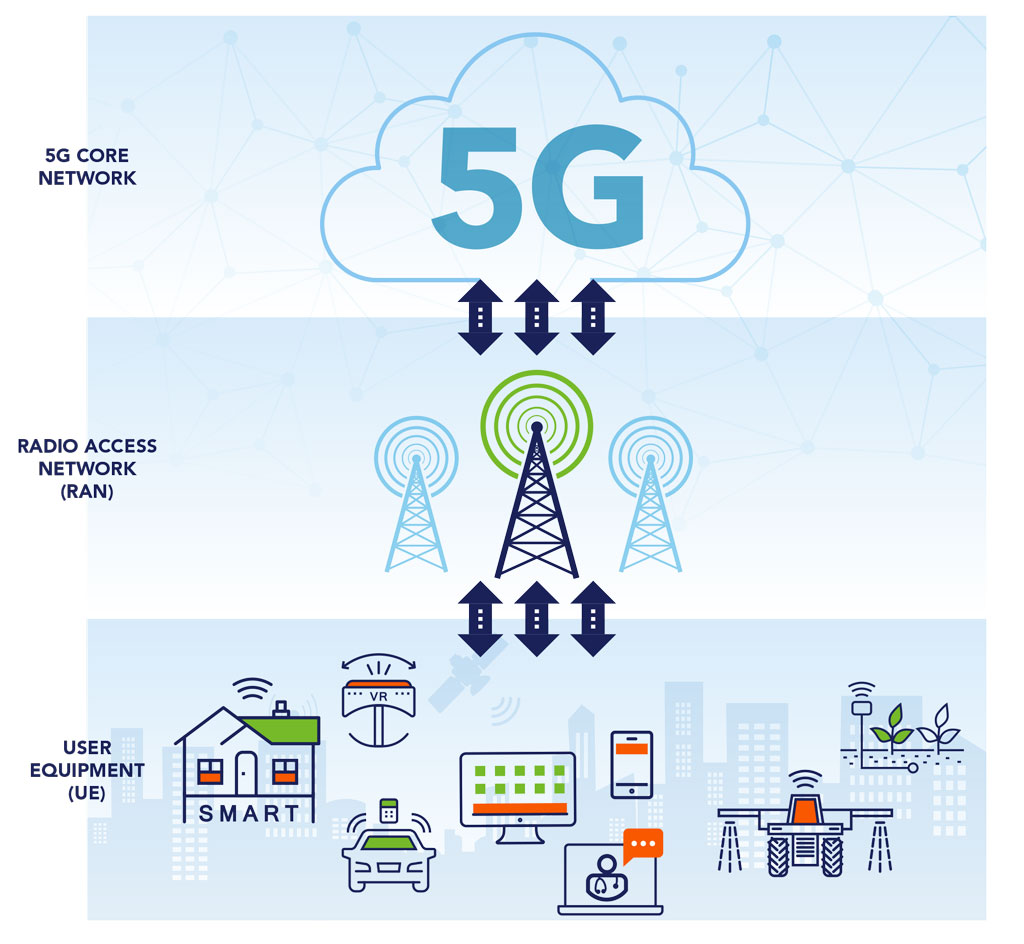
\includegraphics[width=0.5\textwidth]{5G Architecture.jpg}
    \caption{Basic 5G Architecture}
    \label{fig:your_label}
\end{figure}

\section{Data evaluation}

\subsection{Evaluation Methodology}

The evaluation of the collected data was conducted through a series of systematic steps,
designed to accurately measure the networks' adherence to 5G security standards. This
included a detailed analysis of encryption methods, the effectiveness of authentication
schemes, and privacy safeguards.

\subsection{Comparative Analysis}

One of the critical aspects of data evaluation was the comparative analysis between
different networks. This analysis highlighted the variations in security implementation
across various network providers, offering insights into the consistency and reliability
of 5G security practices.

\subsection{Tools and Techniques for Data Evaluation}

The data evaluation phase utilized tools like the commercial analyser Keysight NEMO,
which enabled the researchers to dissect and interpret the complex data sets effectively.
These tools were instrumental in uncovering patterns and discrepancies in security implementations.

\subsection {In-Depth Security Feature Analysis}

The data evaluation process delved into the specifics of various security features
implemented within the 5G networks. This included a thorough examination of end-to-end
encryption protocols, the robustness of identity management and authentication systems,
and the effectiveness of measures designed to protect user privacy. The team employed
advanced analytical methods to dissect and understand the implementation nuances of each
of these security components.

\subsection {Statistical Analysis and Interpretation}

A significant portion of the evaluation involved statistical analysis, where large sets
of data were processed to identify trends, anomalies, and patterns. This analysis was
pivotal in understanding not just the individual implementation of security measures,
but also how these measures performed under different network conditions and user behaviors.

\section {Detailed Results}

The results of the study revealed a multifaceted picture of 5G security in European
networks. While some networks showcased a high degree of compliance with established
security standards, others exhibited notable deficiencies. The variation in the
implementation of security protocols raised concerns about the overall resilience and
reliability of these networks in safeguarding user data.

A key finding was the inconsistency in the deployment of encryption protocols across
different networks. Some networks employed cutting-edge encryption techniques, offering
a high level of data protection, whereas others were found using outdated or less secure
methods. Similarly, the authentication mechanisms varied significantly, with some networks
implementing stringent multi-factor authentication systems, while others had vulnerabilities
that could potentially be exploited.

The study also highlighted uneven practices in privacy measures and data protection
across the surveyed networks. Some networks demonstrated robust systems to ensure user
privacy and data security, incorporating advanced technologies like anonymization and
secure data handling protocols. In contrast, other networks showed lapses in these areas,
posing risks to user privacy and data integrity.

The comparative analysis across different network operators provided critical insights
into the varying levels of security implementation. Tables included in the study
summarized key aspects of this comparison, detailing the performance of each network in
terms of encryption, authentication, and privacy measures.

\begin{table}[h]
	\centering
	\begin{tabular}{|p{0.25\linewidth}|p{0.65\linewidth}|}
		\hline
		\textbf{Attack Area}    & \textbf{Concerns \& Vulnerabilities}                                          \\
		\hline
		Subscriber Credentials  & - Permanent ID exposed (IMSI catching possible).                              \\
		                        & - Temporary IDs can be used for tracking.                                     \\
		\hline
		Authentication Weakness & - Absence of 5G-AKA protocol: users \& services can be inferred.              \\
		                        & - Vulnerabilities in AKA protocol variants.                                   \\
		\hline
		Data Protection         & - Data secrecy present, but integrity missing.                                \\
		                        & - Potential for data alteration and identity attacks.                         \\
		\hline
		Phone Radio Info        & - Risks in sending radio info before full security.                           \\
		                        & - Possible ID, binding, and battery drain attacks, especially for Operator B. \\
		\hline
	\end{tabular}
	\caption{Attack Area Concerns and Vulnerabilities in 5G Networks}
	\label{table:5g-attack-areas}
\end{table}

\section {Detailed discussion}

The discussion section provides a comprehensive analysis of the study's findings, e
mphasizing the crucial role of stringent security measures in the evolving landscape
of 5G networks. The varied implementation of security protocols across different networks highlights a significant challenge in the standardization and enforcement of security practices.

\subsection {Security Implementation Variability}

A primary concern raised by the study is the inconsistency in security implementations. This variability poses a myriad of risks, ranging from data breaches to network vulnerabilities. The study 

\begin{figure}[h]
    \centering
    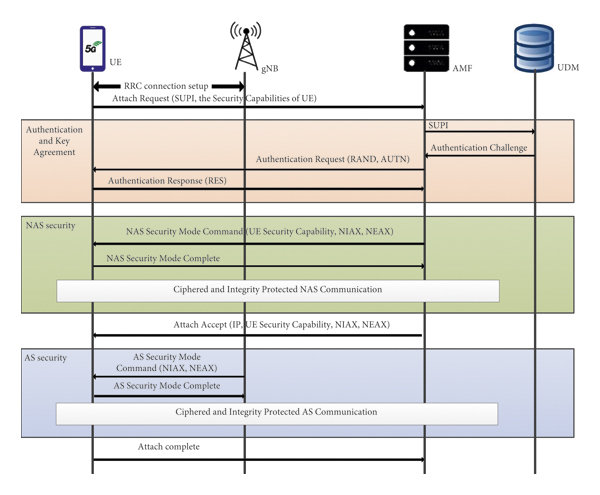
\includegraphics[width=0.5\textwidth]{5G security.png}
    \caption{5G Security Implementation}
    \label{fig:your_label}
\end{figure}

underscores the need for a unified approach to 5G security, advocating for the harmonization of standards and practices across all network providers.

\subsection{Implications for User Privacy and Data Security}

The uneven application of privacy measures and data protection protocols is another critical issue. In an era where data is a valuable commodity, the study emphasizes the need for robust mechanisms to ensure user privacy and data integrity. This includes adopting advanced technologies and best practices in data handling and user authentication.

\subsection {Broader Context and Future Outlook}

The discussion also situates the study's findings within a broader context, considering the rapid evolution of 5G technology and its integration into various aspects of modern life. It highlights the need for ongoing research and adaptation of security measures to keep pace with technological advancements and emerging threats.

\subsection {Challenges in Standardization and Compliance}

One of the major challenges identified is the difficulty in achieving standardization and compliance across diverse network operators. The study calls for more rigorous regulatory frameworks and collaborative efforts among stakeholders to establish and maintain high security standards in 5G networks.

\subsection {Potential for Future Security Enhancements}

Looking ahead, the discussion suggests potential pathways for enhancing 5G security. This includes the development of more sophisticated encryption algorithms, stronger authentication methods, and more comprehensive privacy protection mechanisms. The study advocates for a proactive approach to security, where continuous monitoring and updating of security measures are integral to maintaining the integrity and reliability of 5G networks.

\section {conclusion}

The conclusion of the study synthesizes the key findings and reflections, underscoring the imperative of robust security in the rapidly evolving realm of 5G technology. It acknowledges the significant strides made in developing advanced 5G networks but also highlights the critical gaps and challenges in ensuring their security.

This research makes a substantial contribution to the understanding of 5G security, particularly in the European context. By providing an empirical evaluation of security implementations in real-world scenarios, the study sheds light on the discrepancies between theoretical security models and their practical applications. It offers a valuable benchmark for current security practices and sets a foundation for future enhancements.

A central theme of the conclusion is the urgent need to align theoretical security frameworks with their practical deployment. This alignment is crucial for ensuring the resilience and reliability of 5G networks, especially as they become integral to critical infrastructures and services.

The study concludes with a set of recommendations aimed at network operators, regulatory bodies, and policymakers. These recommendations are focused on closing the gaps identified in the research and enhancing the overall security posture of 5G networks.

There's a call for stronger regulatory frameworks and enforcement mechanisms to ensure uniform adherence to security standards. This includes regular audits, compliance checks, and penalties for non-compliance, fostering a more secure and standardized 5G environment.

The conclusion emphasizes the importance of collaborative efforts among various stakeholders, including network operators, technology providers, and government agencies. Such collaboration is essential for sharing best practices, developing innovative security solutions, and responding effectively to emerging threats.

Finally, the study advocates for continuous research and adaptation of security measures in line with the evolving nature of 5G technology and the changing cyber threat landscape. This includes investing in research and development, staying abreast of the latest security trends, and being proactive in implementing state-of-the-art security technologies.

\section{references}
[1] 3GPP. 2021. TS 33.511: Security Assurance Specification (SCAS) for the next
generation Node B (gNodeB) network product class (Release 16). https://www.
3gpp.org/ftp/Specs/archive/33\{\_\}series/33.511

[2] 3GPP. 2021. TS 38.104: Base Station (BS) radio transmission and reception: Section
5.4.3 Syncronization Raster. https://www.etsi.org/deliver/etsi\_ts/
138100\_138199/138104/15.14.00\_60/ts\_138104v151400p.pdf

[3] 3GPP. 2022. TS 33.501: Security architecture and procedures for 5G system. https://www.3gpp.org/ftp/Specs/archive/33\{\_\}series/33.501/

[4] Ravishankar Borgaonkar et al. 2019. New privacy threat on 3G, 4G, and upcoming
5G AKA protocols. Proceedings on Privacy Enhancing Technologies 2019, 3 (2019).

[5] Ya-Chu Cheng and Chung-An Shen. 2022. A New Tracking-Attack Scenario
Based on the Vulnerability and Privacy Violation of 5G AKA Protocol. IEEE
Access 10 (2022), 77679\textendash{}77687.

[6] Merlin Chlosta et al. 2019. LTE security disabled: misconfiguration in commercial
networks. In Proceedings of the 12th conference on security and privacy in wireless
and mobile networks. 261\textendash{}266.

[7] Merlin Chlosta et al. 2021. 5G SUCI-catchers: still catching them all?. In Proceedings of the 14th ACM Conference on Security and Privacy in Wireless and Mobile
Networks. 359\textendash{}364.

[8] Zhiwei Cui et al. 2022. Security Threats to Voice Services in 5G Standalone
Networks. Security and Communication Networks 2022 (2022).

[9] Adrian Dabrowski et al. 2014. IMSI-catch me if you can: IMSI-catcher-catchers.
https://doi.org/10.1145/2664243.2664272

[10] GSMA. 2022. The future of 5G connectivity in Europe. Product. https://www.

[11] European 5G Security in the Wild: Reality versus Expectations https://arxiv.org/pdf/2305.08635.pdf

\end{document}
\endinput
%%
%% End of file `sample-sigconf.tex'.
